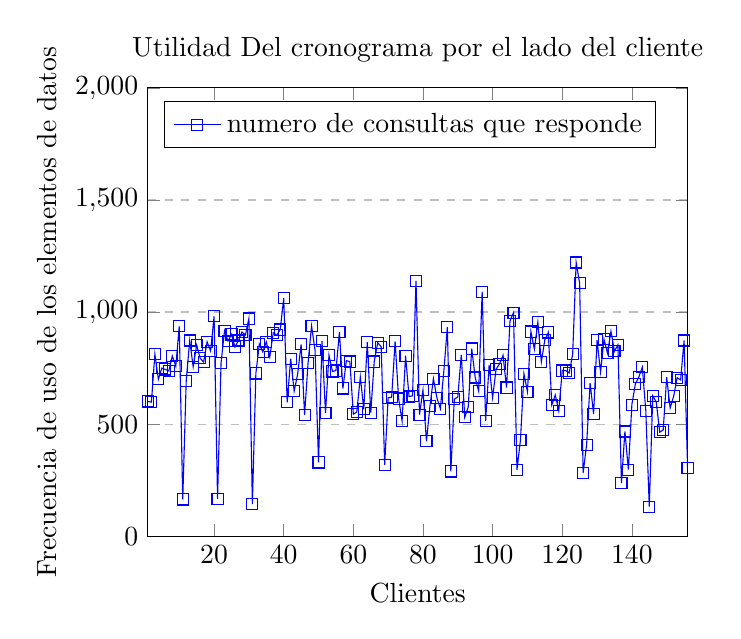
\begin{tikzpicture}
\begin{axis}[
    title={Utilidad Del cronograma por el lado del cliente},
    xlabel={Clientes},
    ylabel={Frecuencia de uso de los elementos de datos},
    xmin=1, xmax=156,
    ymin=0, ymax=2000,
    xtick={},
    ytick={},
    legend pos=north west,
    ymajorgrids=true,
    grid style=dashed,
]

\addplot[
    color=blue,
    mark=square,
    ]
    coordinates {
    %USO EXACTO
    (1,601)
(2,598)
(3,812)
(4,700)
(5,750)
(6,744)
(7,737)
(8,804)
(9,758)
(10,936)
(11,164)
(12,694)
(13,873)
(14,756)
(15,853)
(16,794)
(17,777)
(18,867)
(19,826)
(20,981)
(21,166)
(22,773)
(23,916)
(24,871)
(25,900)
(26,844)
(27,873)
(28,911)
(29,898)
(30,971)
(31,143)
(32,726)
(33,857)
(34,822)
(35,867)
(36,800)
(37,908)
(38,896)
(39,922)
(40,1062)
(41,597)
(42,792)
(43,647)
(44,722)
(45,856)
(46,541)
(47,774)
(48,938)
(49,830)
(50,329)
(51,870)
(52,550)
(53,808)
(54,735)
(55,739)
(56,911)
(57,659)
(58,783)
(59,779)
(60,544)
(61,554)
(62,711)
(63,566)
(64,866)
(65,551)
(66,779)
(67,863)
(68,845)
(69,318)
(70,618)
(71,620)
(72,869)
(73,614)
(74,514)
(75,805)
(76,623)
(77,626)
(78,1139)
(79,542)
(80,652)
(81,423)
(82,581)
(83,703)
(84,617)
(85,569)
(86,738)
(87,933)
(88,289)
(89,611)
(90,621)
(91,809)
(92,530)
(93,577)
(94,837)
(95,708)
(96,647)
(97,1091)
(98,515)
(99,763)
(100,618)
(101,745)
(102,769)
(103,807)
(104,663)
(105,960)
(106,997)
(107,296)
(108,429)
(109,725)
(110,645)
(111,913)
(112,834)
(113,955)
(114,778)
(115,876)
(116,909)
(117,585)
(118,630)
(119,559)
(120,739)
(121,739)
(122,728)
(123,813)
(124,1221)
(125,1128)
(126,282)
(127,408)
(128,684)
(129,545)
(130,874)
(131,733)
(132,878)
(133,817)
(134,914)
(135,825)
(136,854)
(137,237)
(138,467)
(139,297)
(140,587)
(141,679)
(142,710)
(143,754)
(144,560)
(145,132)
(146,626)
(147,599)
(148,464)
(149,474)
(150,709)
(151,572)
(152,624)
(153,707)
(154,697)
(155,873)
(156,305)
(157,630)
    };
    \legend{numero de consultas que responde}

\end{axis}
\end{tikzpicture}

